% Overleaf: upload this file, figures/ and tables/; select pdfLaTeX and Recompile.
\documentclass[10pt,a4paper]{article}
\usepackage[margin=15mm,columnsep=6mm]{geometry}
\usepackage{amsmath,amssymb,graphicx,booktabs}
\usepackage{multicol,caption}
\usepackage[T1]{fontenc}
\usepackage{lmodern}
\usepackage{hyperref}
\hypersetup{colorlinks=true,urlcolor=blue,citecolor=black,linkcolor=black,
  pdftitle={ThermoRL: Occupancy- and Weather-Aware Classroom Cooling},
  pdfauthor={Vyankatesh Deshpande; Rajas Kadu}}
\setlength{\parindent}{0pt}
\setlength{\parskip}{3pt}
\setlength{\emergencystretch}{2em}
\setlength{\textfloatsep}{6pt}
\setlength{\intextsep}{5pt}
\setlength{\abovedisplayskip}{4pt}
\setlength{\belowdisplayskip}{4pt}
\setlength{\abovecaptionskip}{3pt}
\setlength{\belowcaptionskip}{0pt}
\captionsetup{font=small,labelfont=bf,hypcap=false}
\renewcommand{\figurename}{Fig.}
\newcommand{\sect}[1]{\vspace{5pt}\noindent{\large\bfseries #1}\par\vspace{1pt}}
\newcommand{\subhead}[1]{\noindent\textbf{#1}}
\newcommand{\R}{\mathbb{R}}
\begin{document}
\twocolumn[{
\centering
{\LARGE\bfseries ThermoRL: Occupancy- and Weather-Aware\\[2pt]
Classroom Cooling Using Reinforcement Learning\par}
\vspace{5pt}
{\normalsize Vyankatesh Deshpande (B23CS1079)\quad Rajas Kadu (B23CH1039)\par}
\vspace{3pt}
{\small\href{https://github.com/VyankateshD206/AI-Assignment-RL}{github.com/VyankateshD206/AI-Assignment-RL}\par}
\vspace{7pt}
\begin{minipage}{.97\textwidth}\small
\textbf{Abstract.} ThermoRL studies classroom cooling as a sequential resource-allocation
problem: two thermally different rooms compete for a shared electrical allowance.
An original Python simulator supports tabular Q-learning and a deep Q-network
(DQN), with explicit class-arrival, early-class and daily comfort measurements.
We compare frozen agents with three reference controllers on identical synthetic
days. DQN improves arrival comfort over the reactive thermostat, but the timetable
reference achieves better daily comfort with substantially lower energy. The
current experiments do not establish energy-saving superiority of RL.
\end{minipage}
\vspace{8pt}
}]

\sect{1. Problem and environment}
Reactive cooling can leave a room hot when a class starts; excessive precooling
can waste electricity or overcool it. A shared limit couples the decisions:
cooling one room now can prevent service to the other. We investigate whether
reward-driven policies learn this delayed comfort--energy tradeoff.

One episode is a 24-hour day with $H=288$ five-minute decisions
($\Delta t=1/12$ h). Outdoor temperature, solar gain, attendance, class-time jitter
and initial temperatures are seeded synthetic inputs. Announced cancellations
and delays are observable through timetable features. For room $i\in\{1,2\}$,
\begin{align}
T_{i,t+1}={}&T_{i,t}+\frac{\Delta t}{C_i}\big[
U_i(T_t^o-T_{i,t})+g_i I_t \notag\\[-2pt]
&\qquad +0.075n_{i,t}+0.12f_{i,t}-12u_{i,t}\big].
\label{eq:thermal}
\end{align}
Here $u,f\in\{0,1\}$ denote AC and fan operation; $n$ is occupancy and $I$ solar
irradiance. $C=(1.5,1.8)$ kWh/$^{\circ}$C, $U=(0.16,0.14)$ kW/$^{\circ}$C and
$g=(0.003,0.0015)$ kW/(W/m$^2$). AC removes 12 kW of thermal heat while drawing
3 kW electrically; each room's fan group draws 0.12 kW. Initial temperatures are
uniformly sampled from $27$--$30^{\circ}$C. The model is not calibrated to a building.

\sect{2. RL formulation}
We use a finite-horizon discounted control formulation, maximizing
$\mathbb{E}_{\pi}[\sum_{t=0}^{H-1}\gamma^t r_t]$, with $\gamma=0.99$.

\subhead{State and observation space ($\mathcal S$).}
The agent receives $o_t\in\R^{17}$:
\begin{align*}
o_t=(&T_1,T_2,n_1,n_2,\tau_1,\tau_2,n_1^+,n_2^+,T^o,I,\\
&\sin\phi,\cos\phi,B,u_1^-,u_2^-,\tau_B,B^+).
\end{align*}
The entries are room temperatures/occupancies; time and attendance of the next
announced class; weather; cyclical time; current cap; previous AC states; and time
to, and value of, the next cap. Temperatures divide by 50, occupancy by 60,
lookahead minutes (clipped at 240) by 240, irradiance by 1000 and caps by 8.
Binary/cyclical terms retain their natural scale. The underlying simulator state
also contains the generated day's trajectory and clock; these 17 features are
an approximate Markov summary, rather than a proof of full observability.

\subhead{Action space ($\mathcal A$).}
Each room has four modes: off, fan, AC, or AC+fan. The centralized action
$a_t=4m_{1,t}+m_{2,t}\in\{0,\ldots,15\}$ selects both modes jointly. The feasible
set is
\[
\mathcal A_t=\{a:\,\textstyle\sum_i(3u_i+0.12f_i)\le B_t\}.
\]
The normal cap is 6.5 kW; stressed scenarios impose 3.3 kW from 11:00 to 16:00,
preventing simultaneous AC use. Masks constrain exploration, greedy actions and
bootstrap targets. Feasibility is enforced, not learned.

\subhead{Reward function ($\mathcal R$).}
Let $\theta_i=T_{i,t+1}-1.5f_{i,t}$ be the post-action comfort proxy and
$d_i=[23-\theta_i]_+ +[\theta_i-26]_+$, where $[x]_+=\max(x,0)$. Define
\begin{align*}
E_t&=\Delta t\textstyle\sum_i(3u_i+0.12f_i),\\[-2pt]
D_t&=\Delta t\textstyle\sum_i(n_i/60)d_i^2,\\[-2pt]
F_t&=\Delta t\max_i\big(\mathbf1_{n_i>0}d_i^2\big),\quad
K_t=\textstyle\sum_i|u_i-u_i^-|,\\[-2pt]
r_t&=-\big(0.3E_t+2D_t+F_t+0.02K_t\big).
\end{align*}
Energy penalizes all equipment use, including empty-room precooling. Occupancy
weights discomfort; the worst-room term discourages unequal service, and switching
has a small cost. Empty rooms earn no comfort credit. The fixed fan offset is a
comfort assumption, not a physiological model.

\sect{3. Learning algorithms}
\subhead{Tabular Q-learning.}
We discretize two temperatures into six bins each and retain binary occupied,
class-within-30-minutes, cap and previous-AC indicators: at most 4,608 abstract
states. The sparse NumPy table updates
\begin{align*}
\delta&=r+\gamma\max_{a'\in\mathcal A'}Q(s',a')-Q(s,a),\\[-2pt]
Q(s,a)&\leftarrow Q(s,a)+\alpha\delta,
\end{align*}
with $\alpha=0.15$. Terminal targets use $r$ only. Aggregation improves revisitation
but discards useful weather/time detail and can alias distinct conditions.

\subhead{Standard DQN.}
The network maps 21 derived inputs (17 observations with centred temperatures,
plus four hot/cold deviations) through two 64-unit ReLU layers to 16 Q-values.
Following the replay/target-network approach, an Adam optimizer
($3\times10^{-4}$) minimizes Huber loss against
$y=r/10+\gamma\max_{a'\in\mathcal A'}Q_{\bar\omega}(s',a')$; at day end,
$y=r/10$. Replay holds 50,000 transitions, minibatches contain 64, warmup is 500,
and target weights copy every 250 optimizer updates. Gradient norm clips at 10.
Scaling affects numerical units, not the physical reward objective.

\onecolumn
\begin{multicols}{2}
\raggedcolumns
\sect{4. Training and evaluation}
Both agents use feasible-action $\epsilon$-greedy exploration, decaying from 1 to
0.05 over 80\% of training. Four training scenarios cover normal, restricted,
stronger-solar and announced timetable-change conditions. Heatwave ($+4^{\circ}$C)
is excluded. Budgets are 400 DQN and 1,500 Q-learning episodes, precluding an
algorithm-only training-efficiency claim.

Representatives use DQN seed 2 and Q-learning seed 0, with checkpoints 350 and
1350 selected by mean unscaled return on eight validation days
(seeds 1000000--1000001 across four scenarios), checked every 50 episodes.
Figure~\ref{fig:learning} shows stored validation histories, not test curves.
Evaluation freezes weights and Q-values.

\par\smallskip\noindent
\begin{minipage}{\linewidth}
\centering
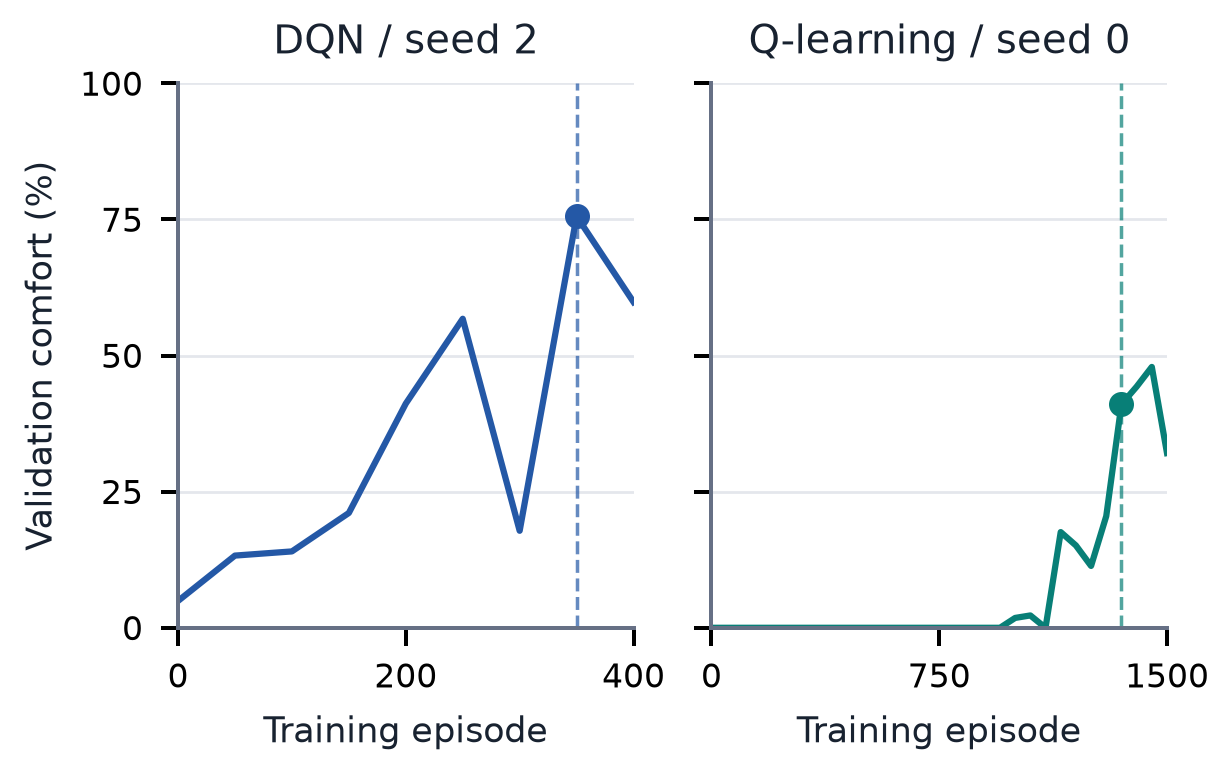
\includegraphics[width=\columnwidth]{figures/learning_curves.png}
\captionof{figure}{Greedy validation comfort on eight fixed days. Dots mark selected
checkpoints. Budgets and horizontal scales differ; these percentages average days.}
\label{fig:learning}
\end{minipage}
\par\smallskip

\subhead{Baselines.}
An occupied-room thermostat uses temperature hysteresis; a timetable controller
also precools 30 minutes before an announced class; rotation alternates priority
every 15 minutes. All receive the same observation and action mask. They are
comparison references only: no imitation labels, supervised pretraining, search
planner or rule-based override is used in the RL agents.

\subhead{Fair comfort measurement.}
\emph{Arrival discomfort} counts occupied class starts outside the band before
the first action, assessing $T_{i,t}-1.5f_{i,t-1}$. \emph{First-15-minute discomfort}
uses uncomfortable occupied room-time at +5, +10 and +15 minutes after a start.
Windows stop at vacancy or a new class and are unioned. \emph{Whole-day comfort}
divides comfortable by occupied room-time. Percentages pool event/minute counts;
energy is mean daily kWh, including all precooling.

\sect{5. Measured results}
Table~\ref{tab:results} and Fig.~\ref{fig:tradeoff} summarize 50 paired synthetic
days per policy: five scenarios, ten seeds each (3000000--3000009), giving
250 policy-days for the five displayed controllers. Conditions and initial
temperatures match across controllers. These are single bundled representatives,
not means over training seeds. This assessment was inspected during a prior
rollback and is now descriptive development evidence, not an untouched final test.

The DQN representative lowers arrival discomfort relative to the reactive
thermostat (28.12\% versus 90.19\%), but uses more than twice its energy and has
slightly poorer daily comfort.

\columnbreak
\par\smallskip\noindent
\begin{minipage}{\linewidth}
\centering
\small
\setlength{\tabcolsep}{2pt}
\renewcommand{\arraystretch}{1.12}
\captionof{table}{Paired 50-day results. Lower arrival/early discomfort and energy are
better; higher whole-day comfort is better. Percentages pool counts.}
\label{tab:results}
% Generated by build_figures.py from data/evaluation_daily.csv.
\begin{tabular}{@{}lrrrr@{}}
\toprule
Policy & \shortstack{Arrival\\discomfort\\(\%)} & \shortstack{Early\\discomfort\\(\%)} & \shortstack{Daily\\comfort\\(\%)} & \shortstack{Energy\\(kWh)}\\
\midrule
Timetable & 31.30 & 8.75 & 92.86 & 24.59\\
Thermostat & 90.19 & 43.94 & 77.49 & 24.05\\
Rotation & 89.92 & 40.94 & 77.47 & 23.54\\
DQN & 28.12 & 22.19 & 75.03 & 50.50\\
Q-learning & 84.62 & 77.81 & 23.16 & 15.52\\
\bottomrule
\end{tabular}

\end{minipage}
\par\smallskip

\par\smallskip\noindent
\begin{minipage}{\linewidth}
\centering
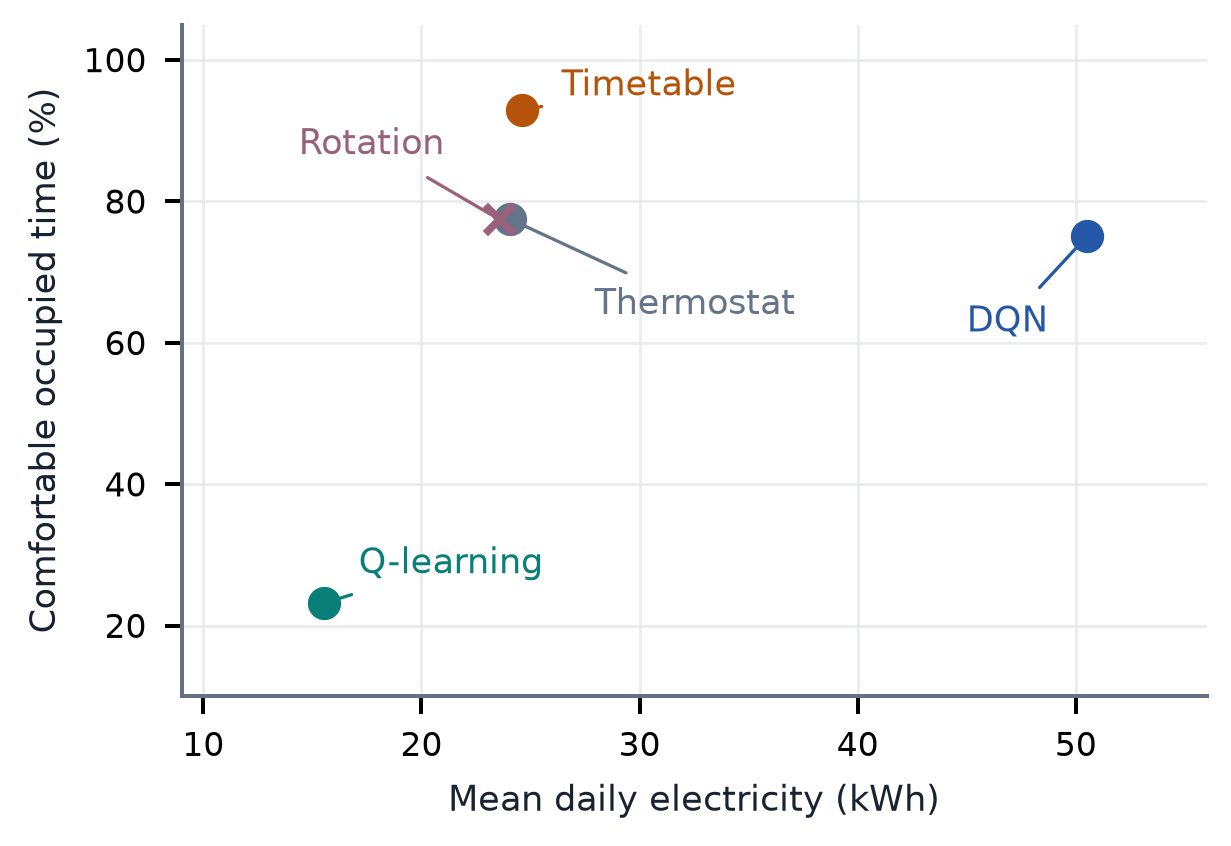
\includegraphics[width=\columnwidth]{figures/energy_comfort.png}
\captionof{figure}{Energy--comfort tradeoff for the same 50 days. The upper-left region
is preferable; low energy with poor comfort is not a successful policy.}
\label{fig:tradeoff}
\end{minipage}
\par\smallskip

Timetable achieves 92.86\% daily comfort at
24.59 kWh; DQN reaches 75.03\% at 50.50 kWh. Q-learning's 15.52 kWh is accompanied
by only 23.16\% comfort, so it does not establish useful savings.

\sect{6. Diagnosis, limitations and outcome}
An 80-day tuning diagnosis attributes 31.93 of the restored DQN's 50.58 kWh/day
to empty-room AC use more than 30 minutes before arrival. This is a diagnostic
signal, not proof of waste. Failure traces also reveal overcooling and prior-fan
effects. Post-action reward and pre-action arrival comfort are distinct quantities.

Nine further 400-episode trials test control, lower learning rate and slower
exploration decay, each with seeds 0/1/2. None preserved all three comfort measures
while reducing energy on 80 tuning days. The previous DQN remains in use;
reserved 100-day confirmation and 100-day final sets remain unused. Failed trials
are retained.

The project contributes shared-budget simulation, original standard RL agents,
arrival-aware assessment and a GUI exposing state, Q-values, masks, transitions
and reward. Results support a reproducible investigation, not RL superiority.
State aliasing, reward alignment and empty-room cooling require further RL
experiments. Synthetic dynamics and few training seeds limit generalization.

\subhead{Reproduction.}
The README supplies installation and exact execution commands. Packaged CSV data
and \texttt{build\_figures.py} regenerate both figures. Reported values were
reproduced from the bundled agents.

\end{multicols}
\end{document}
